\documentclass{article}
\usepackage{graphicx}
\usepackage[margin=1.5cm]{geometry}
\usepackage{amsmath}

\begin{document}
\twocolumn

\title{Friday Warm Up: Unit 1, Capacitors, current and DC circuits}
\author{Prof. Jordan C. Hanson}

\maketitle

\section{Memory Bank}

\begin{itemize}
\item $Q = C\Delta V$ ... Relationship between stored charge, capacitance, and voltage.
\item $I = \Delta Q / \Delta t$ ... The relationship between current, $I$, and charge.
\item $V_{\rm C}(t) = \mathcal{E}\left(1 - \exp(-t/\tau)\right)$ ... The capacitor \textbf{charging} voltage in an RC circuit, with $\tau = RC$.
\item $V_{\rm C}(t) = V_{\rm C,i}\exp(-t/\tau)$ ... The capacitor \textbf{discharging} voltage in an RC circuit, with $\tau = RC$.
\item $\Delta U = Q^2/(2C) = \frac{1}{2}CV^2$ ... Energy stored in a capacitor.
\item $v_{\rm d} = I/(n q A)$ ... Drift velocity of conducting charge.
\item $J = I/A$ ... Current density.
\item $J = \sigma E$ ... Ohm's Law, 1.  $J$ is the current density, and $E$ is the E-field driving current.  The factor $\sigma$ is called the conductivity.  Units: S m$^{-1}$.
\item $\rho = 1/\sigma = E/J$ ... The resistivity.  Units: $\Omega$ m.
\item $V = IR$ ... The macroscopic version of Ohm's law, assuming:
\item $R = L/(\sigma A)$ ... The resistance.  Units: $\Omega$.
\end{itemize}

\section{Capacitors and Energy}

\begin{enumerate}
\item A heart defibrillator being used on a patient has an RC time constant of 10.0 ms due to the resistance of the patient and the capacitance of the defibrillator. (a) If the defibrillator has an 8.00 microfarad capacitance, what is the resistance R of the path through the patient? (b) If the initial voltage is 12.0 kV, how long does it take to decline to 600 V? \\ \vspace{2cm}
\item In the previous exercise, how much energy is delivered to the patient's heart? \\ \vspace{1cm}
\end{enumerate}

\section{DC Current}

\begin{enumerate}
\item What is the drift velocity of charge flowing through a copper wire at 1 A, if the wire has a radius of 5 mm?  For copper, assume that $n = 8.5 \times 10^{28}$ m$^{-3}$. \\ \vspace{3cm}
\item What is the resistance of the wire in the previous exercise, if it is 10 m long?  The resisivity of copper is $1.68 \times 10^{-8}$ $\Omega$ m at 20 degrees C. \\ \vspace{3cm}
\item Consider Fig. \ref{fig:1}.  What is the resistance of the circuit implied by the data?
\end{enumerate}

\begin{figure}
\centering
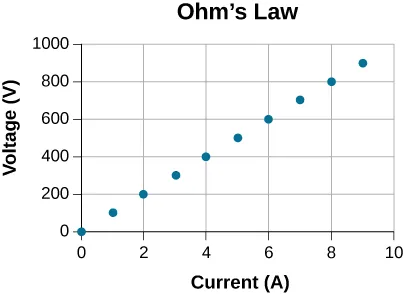
\includegraphics[width=0.33\textwidth]{figures/Ohms.png}
\caption{\label{fig:1} The voltage vs. current in a simple DC circuit.}
\end{figure}

\end{document}
